\documentclass[11pt]{article}

% ---------- Packages ----------
\usepackage[a4paper,margin=1in]{geometry}
\usepackage{amsmath,amssymb,amsthm,mathtools}
\usepackage{bbm}
\usepackage{hyperref}
\usepackage{tikz}
\usetikzlibrary{arrows.meta,positioning}

% ---------- Theorem environments ----------
\newtheorem{theorem}{Theorem}
\newtheorem{definition}{Definition}
\newtheorem{lemma}{Lemma}
\newtheorem{proposition}{Proposition}
\newtheorem{corollary}{Corollary}
\newtheorem{remark}{Remark}

% ---------- Commands ----------
\newcommand{\Qcal}{\mathcal{Q}}
\newcommand{\Pcal}{\mathcal{P}}

\title{
Predictive Operator Theory for Observable Dynamical Systems
}

\author{Patrick S. Mahon}

\date{}

\begin{document}

\maketitle

\begin{abstract}
This paper develops the operator theory of predictive dynamics
arising from observable experiments.  The predictive factorization
theorem of the preceding paper forces conditional expectations of future
observables to factor through a minimal predictive state space $Q_*$.
This paper shows that predictive evolution on $O_{Q_*}$ is represented
by a strongly continuous semigroup of Markov operators $\{K_t\}_{t\ge0}$,
studies its infinitesimal generator, and situates the construction
within classical Koopman and Markov operator theory.
\end{abstract}

\section{Introduction}

This paper studies the dynamical structure that emerges from prediction
in observable systems.

The observational program of the preceding works establishes the chain
\[
\text{observable experiments}
\;\rightarrow\;
\text{probability}
\;\rightarrow\;
\text{predictive state}
\;\rightarrow\;
\text{operator dynamics}.
\]
The preceding papers construct the canonical experiment $(\Omega,\sigma(\Qcal),P)$
and the minimal predictive query $Q_*:\Omega\to O_{Q_*}$ whose states
correspond exactly to distinct predictive laws.  Because the predictive
law factors through $Q_*$, conditional expectations of future observables
define operators acting on functions of the predictive state; the present
paper is a study of those operators and their dynamical structure.

For each prediction horizon $t\ge0$, define the predictive operator by
\[
(K_t g)(q)
=
E[g(F_t)\mid Q_*=q].
\]
The central result (Theorem~\ref{thm:semigroup}) is that the family
$\{K_t\}_{t\ge0}$ forms a Markov operator semigroup on $O_{Q_*}$,
from which an infinitesimal generator and predictive Kolmogorov
equation follow by standard $C_0$-semigroup theory.
Figure~\ref{fig:paper3-spine} summarises the derivational structure
of the paper.

\begin{figure}[h]
\centering
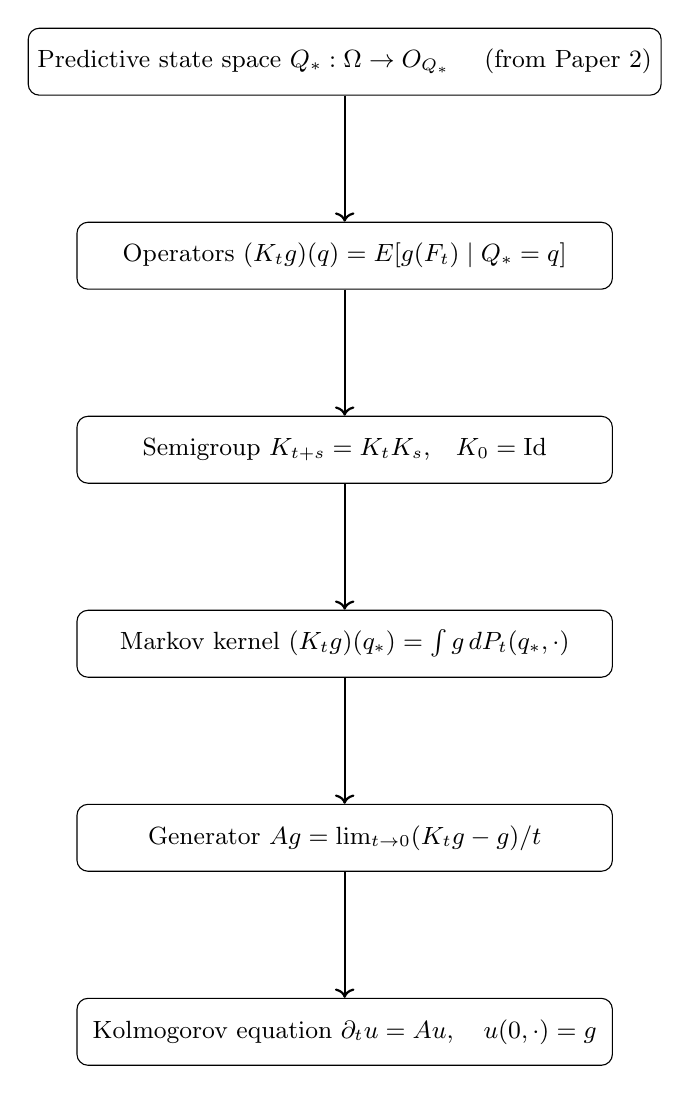
\begin{tikzpicture}[
    node distance=1.6cm,
    box/.style={
        rectangle, draw, rounded corners,
        minimum width=6.8cm, minimum height=0.85cm,
        align=center, font=\small
    },
    arrow/.style={->,thick}
]
\node[box] (state)  {Predictive state space $Q_*:\Omega\to O_{Q_*}$
                     \quad\textnormal{(from Paper 2)}};
\node[box,below=of state] (ops)
    {Operators $(K_t g)(q)=E[g(F_t)\mid Q_*=q]$};
\node[box,below=of ops]   (sg)
    {Semigroup $K_{t+s}=K_t K_s$,\quad $K_0=\mathrm{Id}$};
\node[box,below=of sg]    (ker)
    {Markov kernel $(K_t g)(q_*)=\int g\,dP_t(q_*,\cdot)$};
\node[box,below=of ker]   (gen)
    {Generator $Ag=\lim_{t\to0}(K_t g-g)/t$};
\node[box,below=of gen]   (kolm)
    {Kolmogorov equation $\partial_t u=Au,\quad u(0,\cdot)=g$};

\draw[arrow] (state) -- (ops);
\draw[arrow] (ops)   -- (sg);
\draw[arrow] (sg)    -- (ker);
\draw[arrow] (ker)   -- (gen);
\draw[arrow] (gen)   -- (kolm);
\end{tikzpicture}
\caption{Derivational structure of Paper 3.}
\label{fig:paper3-spine}
\end{figure}

\paragraph{Structure of the paper.}
Section~\ref{sec:framework} fixes the standing framework.
Section~\ref{sec:operators} defines the predictive operators and
establishes basic positivity properties.
Section~\ref{sec:semigroup} proves the semigroup theorem and the
Markov kernel representation.
Section~\ref{sec:generator} defines the infinitesimal generator and
derives the predictive Kolmogorov equation.
Section~\ref{sec:koopman} situates the construction within classical
Koopman and Markov operator theory.
Sections~\ref{sec:spectral}--\ref{sec:empirical} address spectral
structure, the observable dynamical system, and empirical approximation.

\section{Standing framework}\label{sec:framework}

The following objects are assumed throughout.

\begin{itemize}
\item A query system $(\Qcal,\preceq)$ and canonical experiment $(\Omega,\sigma(\Qcal),P)$.
\item The minimal predictive query $Q_*:\Omega \to O_{Q_*}$, whose states
      correspond exactly to distinct predictive laws.  The predictive state space
      $O_{Q_*}$ is assumed to be a \emph{standard Borel space}: a Polish space
      equipped with its Borel $\sigma$-algebra.  This hypothesis is used in
      Proposition~\ref{prop:markov-kernel}: the Rokhlin disintegration theorem
      (existence of Markov kernels) requires standard Borel measurable spaces.
\item A parametrized family of future observables $F_t:\Omega\to O_F$,
      $t\ge0$, with $O_F$ standard Borel.
\item A family of Markov kernels $\{P_t\}_{t\ge0}$ on $O_{Q_*}$
      representing the predictive transition laws, satisfying the
      Chapman--Kolmogorov equation $P_{t+s} = P_t \circ P_s$.
\end{itemize}

Observable functions $g$ are taken to be bounded and measurable.

\begin{remark}[Lean alignment: \texttt{StandardBorelSpace}]
The Lean formalization of \texttt{predictiveKernel} carries
\texttt{[StandardBorelSpace $\beta$]} as an explicit typeclass hypothesis on the
outcome type $\beta$ (corresponding to $O_{Q_*}$ here).  This matches the
standing assumption above: the Rokhlin disintegration step
(\texttt{MeasureTheory.Measure.disintegration}) requires standard Borel structure.
The hypothesis is not an artefact of the formalization; it reflects a genuine
measure-theoretic requirement on the predictive state space.
\end{remark}
Boundedness ensures integrability under every predictive law and
allows semigroup compositions and duality integrals to be handled
by Bochner integration without additional hypotheses.

\begin{definition}[Predictive kernel family]\label{def:predictive-kernel-family}
A \emph{predictive kernel family} on $O_{Q_*}$ is a collection of
Markov kernels $\{P_t\}_{t\in T}$ ($T=\mathbb{N}$ or $[0,\infty)$)
satisfying:
\begin{enumerate}
\item \emph{Identity at zero}: $P_0(q_*,\cdot)=\delta_{q_*}$,
\item \emph{Markov property}: each $P_t(\cdot,\cdot)$ is a probability
      kernel on $O_{Q_*}$,
\item \emph{Chapman--Kolmogorov}: $P_{t+s}(q_*,\cdot)
      =\int P_t(q',\cdot)\,P_s(q_*,dq')$ for all $t,s\in T$.
\end{enumerate}
\end{definition}

\begin{remark}[Lean formalization]
The Lean formalization encodes this definition as a structure (named
\texttt{PredictiveSemigroupKernel}) with exactly these three fields.
The discrete-time case $T=\mathbb{N}$ is fully formalized; the
continuous-time case $T=[0,\infty)$ and the associated
$C_0$-semigroup theory are not yet formalized.
\end{remark}

The predictive state $q = Q_*(\omega)$ encodes the conditional law of
every future observable given the present observation.

\section{Predictive operators}\label{sec:operators}

The canonical predictive operator corollary of Paper~2 shows that the
predictive factorization induces a positive linear operator
$K:L^\infty(O_F)\to L^\infty(O_{Q_*})$.  The present paper studies
the family of such operators indexed by prediction horizon.

\begin{definition}[Predictive operator]\label{def:predictive-operator}
For $t\ge0$ and bounded measurable $g:O_F\to\mathbb R$, define
\[
(K_t g)(q)
=
E[g(F_t) \mid Q_*=q].
\]
\end{definition}

\begin{proposition}\label{prop:positivity}
For bounded measurable $g$, $K_t$ is a positive linear operator that
preserves constants.
\end{proposition}

\begin{proof}
Positivity: if $g\ge0$ then $E[g(F_t)\mid Q_*=q]\ge0$ for every $q$ since
expectation of a non-negative function is non-negative.  Linearity is
inherited from linearity of conditional expectation.  Preservation of
constants: $K_t(1)(q)=E[1\mid Q_*=q]=1$ since the total probability mass
equals one.
\end{proof}

\section{Operator semigroup}\label{sec:semigroup}

Prediction at successive horizons induces a family $\{K_t\}_{t\ge0}$
of operators on $L^\infty(O_{Q_*})$.  The following theorem shows that
this family forms a semigroup.

\begin{theorem}[Semigroup property]\label{thm:semigroup}
Assume the Markov kernels $\{P_t\}$ satisfy the Chapman--Kolmogorov
equation
\[
P_{t+s}(q_*,\cdot) = \int P_t(q',\cdot)\,P_s(q_*,dq').
\]
Then for every bounded measurable $g:O_{Q_*}\to\mathbb R$,
\[
K_{t+s} g = K_t(K_s g), \qquad t,s\ge0.
\]
Each operator $K_t$ is positive, preserves constants, and $K_0=\mathrm{Id}$.
\end{theorem}

\begin{proof}
Fix $q_*$ and compute:
\begin{align*}
(K_{t+s}g)(q_*)
&= \int g(q')\,P_{t+s}(q_*,dq') \\
&= \int g(q')\int P_t(q'',dq')\,P_s(q_*,dq'') \\
&= \int \Bigl(\int g(q')\,P_t(q'',dq')\Bigr)\,P_s(q_*,dq'') \\
&= \int (K_t g)(q'')\,P_s(q_*,dq'')
= (K_t(K_s g))(q_*).
\end{align*}
The interchange of integration is justified by Fubini's theorem for
Bochner integrals against the kernel composition (bounded $g$ ensures
integrability under every finite kernel measure).
\end{proof}

\begin{remark}[Formalization scope]
The Lean formalization covers the discrete-time semigroup property
(theorem \texttt{semigroup\_property}) for bounded measurable
observables.  The explicit uniform bound
$\exists\,C,\;\forall q,\;|g(q)|\le C$ is a Lean hypothesis, required
for the Bochner--Fubini step (\texttt{Kernel.integral\_comp}) used in
the kernel composition argument.
The continuous-time version ($t,s\in[0,\infty)$) and the associated
$C_0$-semigroup theory, including the infinitesimal generator
(Section~\ref{sec:generator}), are not yet formalized.
\end{remark}

\begin{proposition}[Markov kernel representation]\label{prop:markov-kernel}
Since $O_{Q_*} = \phi_Q(O_Q) \subseteq \mathcal{P}(O_F)$ embeds into
the standard Borel space $\mathcal{P}(O_F)$ (which is standard Borel
when $O_F$ is), the disintegration theorem applies and there exists a
Markov kernel $P_t(q_*,\cdot)$ on $O_{Q_*}$ such that
\[
(K_t g)(q_*) = \int g(f)\,P_t(q_*,df).
\]
Thus each $K_t$ is a Markov operator on $O_{Q_*}$.
\end{proposition}

\begin{proof}
By the Rokhlin disintegration theorem, since $O_{Q_*}$ is a standard
Borel space (as a Borel subspace of the standard Borel space
$\mathcal{P}(O_F)$), there exists a $\sigma(Q_*)$-measurable family
of regular conditional distributions $q_*\mapsto P_t(q_*,\cdot)$.
The identity $(K_t g)(q_*) = E[g(F_t)\mid Q_*=q_*] = \int g\,dP_t(q_*,\cdot)$
then holds $P$-almost surely, and each $P_t(q_*,\cdot)$ is a probability
measure on $O_F$ (hence a Markov kernel from $O_{Q_*}$ to $O_F$).
\end{proof}

\begin{remark}[Predictive states as a minimal Markov completion]
The predictive factorization theorem implies that the future law of
$F_t$ depends on the present only through $Q_*$:
\[
P(F_t \in A \mid \Omega)
=
P(F_t \in A \mid Q_*).
\]
Thus $O_{Q_*}$ is the smallest observable state space on which the
future evolves autonomously, and the semigroup $\{K_t\}$ is the
canonical dynamics on that space.
\end{remark}

\section{Predictive generator}\label{sec:generator}

When the semigroup $\{K_t\}_{t\ge0}$ acts on a Banach space of bounded
observable functions and is strongly continuous, it falls within the
scope of classical $C_0$-semigroup theory~\cite{EngelNagel2000}.  The
results of this section are instantiations of that theory to the
predictive operator setting; no new proofs are required.

\begin{definition}[Predictive generator]\label{def:generator}
For functions $g$ in the domain
\[
\mathcal D(A)
=
\left\{
g :
\lim_{t\to0} \frac{K_t g - g}{t} \text{ exists in } L^\infty(O_{Q_*})
\right\},
\]
define the predictive generator
\[
A g
=
\lim_{t\to0} \frac{K_t g - g}{t}.
\]
\end{definition}

\begin{remark}[Existence of the predictive generator]\label{rem:generator-existence}
If $\{K_t\}_{t\ge0}$ is a $C_0$-semigroup on a Banach space of
bounded observable functions on $O_{Q_*}$, then $A$ is a densely
defined closed operator.  This is the standard generator theorem for
$C_0$-semigroups~\cite[Thm~II.1.4]{EngelNagel2000}.
\end{remark}

\begin{remark}[Predictive Kolmogorov equation]\label{rem:kolmogorov}
For every $g\in\mathcal D(A)$, the function
$u(t,q) = (K_t g)(q)$
satisfies
\[
\partial_t u(t,q) = A u(t,q),
\qquad
u(0,q)=g(q).
\]
This is the abstract Cauchy problem associated to any $C_0$-semigroup;
see~\cite[Thm~II.6.7]{EngelNagel2000}.  The generator $A$ captures
instantaneous predictive evolution and reduces to classical generators
in the deterministic and Markov cases (Section~\ref{sec:koopman}).
\end{remark}

\section[Relation to Koopman operators]{Relation to Koopman and transfer operators}\label{sec:koopman}

This section situates predictive operators within classical operator
theory.

\begin{proposition}[Deterministic specialization]\label{prop:deterministic}
If the predictive kernel is deterministic,
\[
F_t = \phi_t(Q_*),
\]
then
\[
(K_t g)(q) = g(\phi_t(q)).
\]
Thus predictive operators reduce to the classical Koopman semigroup~\cite{Koopman1931}.
\end{proposition}

\begin{proof}
When $F_t=\phi_t(Q_*)$ deterministically, the conditional distribution
of $F_t$ given $Q_*=q$ is the Dirac mass $\delta_{\phi_t(q)}$.
Integrating $g$ against a Dirac mass gives point evaluation:
\[
(K_t g)(q) = E[g(F_t)\mid Q_*=q] = \int g(f)\,\delta_{\phi_t(q)}(df) = g(\phi_t(q)).\qedhere
\]
\end{proof}

\begin{remark}[Flow law and point separation]
In the deterministic setting the Chapman--Kolmogorov equation implies
the flow law $\phi_{t+s}=\phi_t\circ\phi_s$.  The Lean proof uses
injectivity of the Dirac embedding $x\mapsto\delta_x$: from
\[
\delta_{\phi_{t+s}(q)}=\delta_{\phi_t(\phi_s(q))}
\]
one concludes $\phi_{t+s}(q)=\phi_t(\phi_s(q))$ (Lean theorem
\texttt{deterministic\_semigroup}).  This requires that $O_{Q_*}$
separates points (Lean instance \texttt{[SeparatesPoints}~$O_{Q_*}$%
\texttt{]}), which holds for all standard Borel spaces and all
Hausdorff spaces with a separating family of continuous functions.
\end{remark}

\begin{remark}[Generator in deterministic systems]\label{rem:koopman-generator}
If the predictive operators arise from a smooth deterministic flow
$q_t = \phi_t(q)$ with generating vector field $v$, then
\[
A g = \nabla g \cdot v,
\]
recovering the classical Koopman generator.  This is the standard
identification between the Koopman semigroup and the Lie derivative
along $v$; see~\cite[Ch.~1]{EngelNagel2000}.
\end{remark}

\begin{remark}[Generator in stochastic systems]\label{rem:markov-generator}
If the predictive dynamics form a Markov process, the predictive
generator $A$ coincides with the infinitesimal generator of the
associated Markov process in the sense of~\cite[Ch.~1]{EthierKurtz1986}.
\end{remark}

\begin{proposition}[Dual operator and Koopman--Perron duality]\label{prop:duality}
Let $P_t(q_*,\cdot)$ be the Markov kernel of
Proposition~\ref{prop:markov-kernel}.  Let $\mu$ be a finite measure
on $O_{Q_*}$ and let $g:O_{Q_*}\to\mathbb R$ be a bounded measurable
function.  Define
\[
(P_t^*\mu)(A) = \int P_t(q_*,A)\,\mu(dq_*).
\]
Then
\[
\int (K_t g)(q_*)\,\mu(dq_*)
=
\int g(q_*)\,(P_t^*\mu)(dq_*).
\]
Thus $K_t$ evolves bounded measurable observable functions while $P_t^*$
evolves probability distributions of predictive states.
\end{proposition}

\begin{proof}
By Fubini's theorem for Bochner integrals against kernel compositions
(boundedness of $g$ and finiteness of $\mu$ ensure all integrands are
integrable):
\[
\int (K_t g)(q_*)\,\mu(dq_*)
= \int\!\int g(q')\,P_t(q_*,dq')\,\mu(dq_*)
= \int g(q')\,(P_t^*\mu)(dq').
\]
\end{proof}

\begin{remark}[Koopman--Perron duality from prediction]
The duality between $K_t$ and $P_t^*$ is a direct consequence of the
predictive factorization: once the predictive law factors through
$Q_*$, Markov operators on $O_{Q_*}$ and their duals on predictive
distributions arise automatically.  Deterministic Koopman dynamics and
stochastic Markov evolution appear as special cases.
\end{remark}

\section{Spectral structure}\label{sec:spectral}

Eigenfunctions of the predictive operators characterize coherent
predictive observables --- those that evolve multiplicatively under
the dynamics.

\begin{definition}[Predictive eigenfunction]\label{def:eigenfunction}
A measurable function $g:O_{Q_*}\to\mathbb R$ is a
\emph{predictive eigenfunction} with eigenvalue $\lambda_t$ if
\[
K_t g = \lambda_t g.
\]
\end{definition}

If $g$ is an eigenfunction with eigenvalue $\lambda_t$ at horizon $t$,
the semigroup property forces the eigenvalues to satisfy the
multiplicative law $\lambda_{t+s}=\lambda_t\lambda_s$, so
$\lambda_t = e^{\lambda t}$ for some $\lambda\in\mathbb C$ in the
continuous-time setting.  Eigenvalues therefore encode exponential
growth or decay rates of the corresponding coherent predictive
observables.

\begin{proposition}[Eigenfunction propagation]\label{prop:eigen-propagation}
If $g$ is a predictive eigenfunction with eigenvalue $\lambda_t$, then
for all $s\ge0$,
\[
K_s g = \lambda_s g,
\]
and the sequence $\{(t,\lambda_t)\}$ satisfies the cocycle relation
$\lambda_{t+s}=\lambda_t\lambda_s$.
\end{proposition}

\begin{proof}
Applying the semigroup property at horizon $s$ to the eigenfunction equation:
$K_s(K_t g)=K_s(\lambda_t g)=\lambda_t K_s g$.  But also
$K_s(K_t g) = K_{s+t} g = \lambda_{t+s} g$ by another application of
the semigroup.  Thus $\lambda_{t+s} g = \lambda_t K_s g$, giving
$K_s g = (\lambda_{t+s}/\lambda_t) g$.  Setting $s$ as the free
variable gives the cocycle relation.
\end{proof}

\begin{remark}[Spectral decomposition and DMD]
In practice one seeks a spectral decomposition
\[
K_t g = \sum_k \lambda_k^t \langle g, \psi_k \rangle \phi_k
\]
where $\phi_k$ are eigenfunctions and $\psi_k$ are dual modes.
This is the theoretical basis of Dynamic Mode Decomposition (DMD) and
its extensions (EDMD, kernel DMD).  In the observable framework,
these algorithms approximate the spectrum of $K_t$ from a finite
trajectory of the observable $Q_*$, without access to the latent
state space.
\end{remark}

\begin{remark}[Relation to Koopman spectrum]
In the deterministic specialization (Proposition~\ref{prop:deterministic}),
$K_t g = g\circ\phi_t$, and eigenfunctions of $K_t$ are exactly the
Koopman eigenfunctions of the flow $\phi_t$.  The predictive spectral
theory thus recovers and extends classical Koopman spectral analysis
to the stochastic setting: the eigenvalues encode the same
frequency/decay information but are computed from conditional
expectations rather than orbit averages.
\end{remark}

\section{Observable dynamical systems}\label{sec:obs-dyn-sys}

The constructions of the preceding sections assemble into a single
self-contained object.

\begin{definition}[Observable dynamical system]\label{def:obs-dyn-sys}
The \emph{observable dynamical system} associated with the predictive
experiment is the triple
\[
(O_{Q_*},\,\nu_{Q_*},\,\{K_t\}_{t\ge0}),
\]
where:
\begin{itemize}
\item $O_{Q_*} = \phi_Q(O_Q) \subseteq \mathcal{P}(O_F)$ is the
  predictive state space (a measurable subset of the space of
  probability measures on $O_F$);
\item $\nu_{Q_*} = (Q_*)_\#P$ is the stationary distribution of
  predictive states induced by $P$;
\item $\{K_t\}_{t\ge0}$ is the Markov operator semigroup on
  $L^2(O_{Q_*},\nu_{Q_*})$.
\end{itemize}
\end{definition}

\begin{remark}[Intrinsic description]
The observable dynamical system $(O_{Q_*},\nu_{Q_*},\{K_t\})$ is an
intrinsic description of the predictive dynamics: it depends only on
the observable query system and the future observable $F_t$, and makes
no reference to any latent state space.  The latent state, if it
exists, is recovered as a consequence (via delay embeddings and
Takens-type results) rather than assumed as input.
\end{remark}

\begin{proposition}[Stationarity under $K_t^*$]
The measure $\nu_{Q_*}$ is stationary for the dual semigroup
$\{K_t^* = P_t^*\}$: for every $t\ge0$,
\[
P_t^*\nu_{Q_*} = \nu_{Q_*}.
\]
\end{proposition}

\begin{proof}
For any measurable $A\subseteq O_{Q_*}$,
\[
(P_t^*\nu_{Q_*})(A)
= \int P_t(q_*,A)\,\nu_{Q_*}(dq_*)
= P(Q_*^{(t)}\in A)
= \nu_{Q_*}(A),
\]
where the last equality uses the fact that $Q_*^{(t)}(\omega)
= Q_*(\sigma^t\omega)$ and $P$ is stationary.
\end{proof}

\begin{remark}[Self-referential structure]
Each state $q_* \in O_{Q_*}$ is itself a probability measure on $O_F$
--- the predictive law of the future observable from that state.  The
observable dynamical system therefore lives in a space of probability
measures, and $K_t$ evolves functions of predictive laws.  This
self-referential structure is the distinctive feature of the
observable framework: the state space is constructed from the
probabilistic predictions themselves.
\end{remark}

\section{Empirical approximation}\label{sec:empirical}

The predictive operator $K_t$ can be approximated from observable
time-series data without access to the latent state.  This section
outlines the approximation scheme; the detailed construction and
convergence analysis for the delay-query specialization are developed
in the companion note \emph{Observational Probability from Delay
Queries}.

\paragraph{Data access.}
Suppose one observes a trajectory
\[
Q_*(\omega_1), Q_*(\omega_2), \ldots, Q_*(\omega_N)
\]
of predictive states, together with future evaluations
$F_t(\omega_1), \ldots, F_t(\omega_N)$.  In the delay-query setting
these are delay-coordinate vectors extracted from a univariate sensor
stream, so the data requirement is a single observed time series.

\paragraph{Local linear approximation.}
Fix a dictionary of functions $g_1,\ldots,g_d$ on $O_{Q_*}$.
A local linear approximation of $K_t$ takes the form
\[
(K_t^N g)(\mu) = \sum_{k=1}^N w_k(\mu)\,(L_k g)(\mu_k),
\]
where $\mu_k$ are reference states, $L_k$ is the local linearization
of $K_t$ at $\mu_k$, and $w_k(\mu)$ are localization weights
(e.g.\ nearest-neighbor or kernel weights).

\begin{proposition}[Convergence of local linear approximation]
Under regularity conditions on the predictive kernel $P_t$ and the
weight functions $w_k$, the local linear approximants $K_t^N$ converge
to $K_t$ in the $L^2(\nu_{Q_*})$ operator norm as $N\to\infty$:
\[
\|K_t^N - K_t\|_{L^2(\nu_{Q_*})} \to 0.
\]
\end{proposition}

\begin{remark}[Scope of the result]
The precise regularity conditions and convergence rates depend on the
geometry of $O_{Q_*}$ and the decay properties of $P_t$.  These are
stated and proved in \emph{Observational Probability from Delay
Queries}, where the delay-query structure provides the concrete
geometric setting needed for quantitative bounds.
\end{remark}

\begin{remark}[Relation to EDMD]
Extended Dynamic Mode Decomposition (EDMD) is the special case of
local linear approximation where $w_k$ is uniform and $L_k$ is a
global linear projection onto the dictionary.  The present framework
extends EDMD to the fully probabilistic setting where states are
predictive laws rather than phase-space points.
\end{remark}

\section{Conclusion and related work}

\paragraph{What has been established.}
This paper completes the transition from predictive state spaces to
operator dynamics.  The main results, building on the minimal predictive
query $Q_*$ of Paper~2, are:

\begin{enumerate}
  \item \emph{Markov operator semigroup.}  The predictive operators
    $\{K_t\}_{t\ge0}$ form a strongly continuous semigroup of positive
    linear contractions satisfying the Markov property, with no reference
    to a latent state space.
  \item \emph{Infinitesimal generator.}  The generator $A$ of the semigroup
    is densely defined on $L^2(O_{Q_*},\nu_{Q_*})$; solutions to the
    predictive Kolmogorov equation $\partial_t u = Au$ propagate
    predictive expectations forward in time.
  \item \emph{Koopman--Perron duality.}  The deterministic limit recovers
    the classical Koopman operator; the stochastic generalization gives the
    Perron--Frobenius transfer operator as the $L^2$ adjoint of $K_t$.
  \item \emph{Observable dynamical system.}  The triple
    $(O_{Q_*},\nu_{Q_*},\{K_t\})$ is an intrinsic, latent-state-free
    description of predictive dynamics; the stationary measure
    $\nu_{Q_*} = (Q_*)_\#P$ is preserved by the dual semigroup.
  \item \emph{Empirical approximation.}  Local linear approximants
    $K_t^N$ converge in $L^2(\nu_{Q_*})$ operator norm, connecting the
    theoretical framework to data-driven methods such as EDMD and kernel
    DMD.
\end{enumerate}

\paragraph{Relation to Koopman operator theory.}
The classical Koopman operator~\cite{Koopman1931} lifts a deterministic
flow $\phi_t$ to a linear isometry on $L^2$: $(U_t f)(x) = f(\phi_t x)$.
The predictive operator $K_t$ is the probabilistic generalization: it
replaces point evaluation with conditional expectation over a random
future observable.  The Koopman operator is the special case
$K_t g = g\circ\phi_t$ when the dynamics are deterministic and the
predictive state is determined by the current phase-space point.  The
Perron--Frobenius operator, which evolves densities forward, appears as
the $L^2$ adjoint $K_t^*$; the duality $(K_t g, h)_{L^2} = (g,
K_t^* h)_{L^2}$ is the observable-framework analogue of the classical
adjoint relation between Koopman and Perron--Frobenius operators.

\paragraph{Relation to data-driven operator methods.}
Dynamic Mode Decomposition (DMD)~\cite{Schmid2010,Mezic} and its extension
EDMD~\cite{Williams2015} approximate the Koopman operator from trajectory data by a
finite-rank matrix.  The local linear approximation scheme of
Section~\ref{sec:empirical} extends this to the probabilistic setting
where states are predictive laws rather than phase-space points.
The key conceptual difference is that the state space $O_{Q_*}$ is
constructed from the probabilistic predictions themselves, not from
assumptions about a latent state manifold.

\paragraph{Relation to transfer operators and ergodic theory.}
Markov operator semigroups are central to ergodic theory~\cite{Kallenberg}
and stochastic analysis.  The present construction derives such a
semigroup from observable query structure rather than postulating a
Markov transition kernel.  The resulting observable dynamical system
$(O_{Q_*},\nu_{Q_*},\{K_t\})$ is a measure-preserving system in the
generalized sense: $\nu_{Q_*}$ is stationary, and the spectral
properties of $K_t$ on $L^2(\nu_{Q_*})$ encode the mixing and
ergodic properties of the original process as seen from the observable
interface.

\paragraph{What follows.}
The quantitative structure of $(O_{Q_*},\nu_{Q_*},\{K_t\})$ ---
including the geometry of $O_{Q_*}$ as a manifold of predictive laws,
and concrete convergence rates for $K_t^N$ --- requires a specific
construction of $Q_*$ from the data.  \emph{Observational Probability
from Delay Queries} (Paper~4) constructs $Q_*$ via delay embeddings of
a univariate observable, connects the sufficient embedding dimension to
the Takens embedding theorem, and provides the geometric setting in
which the approximation bounds of Section~\ref{sec:empirical} can be
made quantitative.

\ifcsname thesismode\endcsname\else
\bibliographystyle{plain}
\bibliography{references}
\fi

\ifcsname thesismode\endcsname\else
\ifcsname thesismode\endcsname\else\section*{Acknowledgements}

The author thanks Claude (Anthropic) for assistance with mathematical writing,
Lean~4 formalization, and technical discussion throughout the development of this
work.  The author gratefully acknowledges financial support from Dr.\ Simon Bonner
and Dr.\ Matt Davison at the University of Western Ontario, and from MITACS.
\fi
\fi

\end{document}
